\section{Android application}\label{sec:app_plans}
We implement the Android application "SwimPredictor" using Java, a minimum SDK version of 22 and a target SDK version of 28. The app implements three functionalities: The usage of the trained models, a stopwatch to measure the times and a database to store the predicted results and swimmer information to access it later when he makes the competition registration. All three functionalities are implemented as fragments and can be accessed from a bottom tab navigation whats makes changing from one functionality to another very easy and intuitive. Figure \ref{fig:app_screenshots} shows screenshots of the final Android application.\\
\begin{figure}[ht]
\centering
\begin{minipage}{0.2\textwidth}
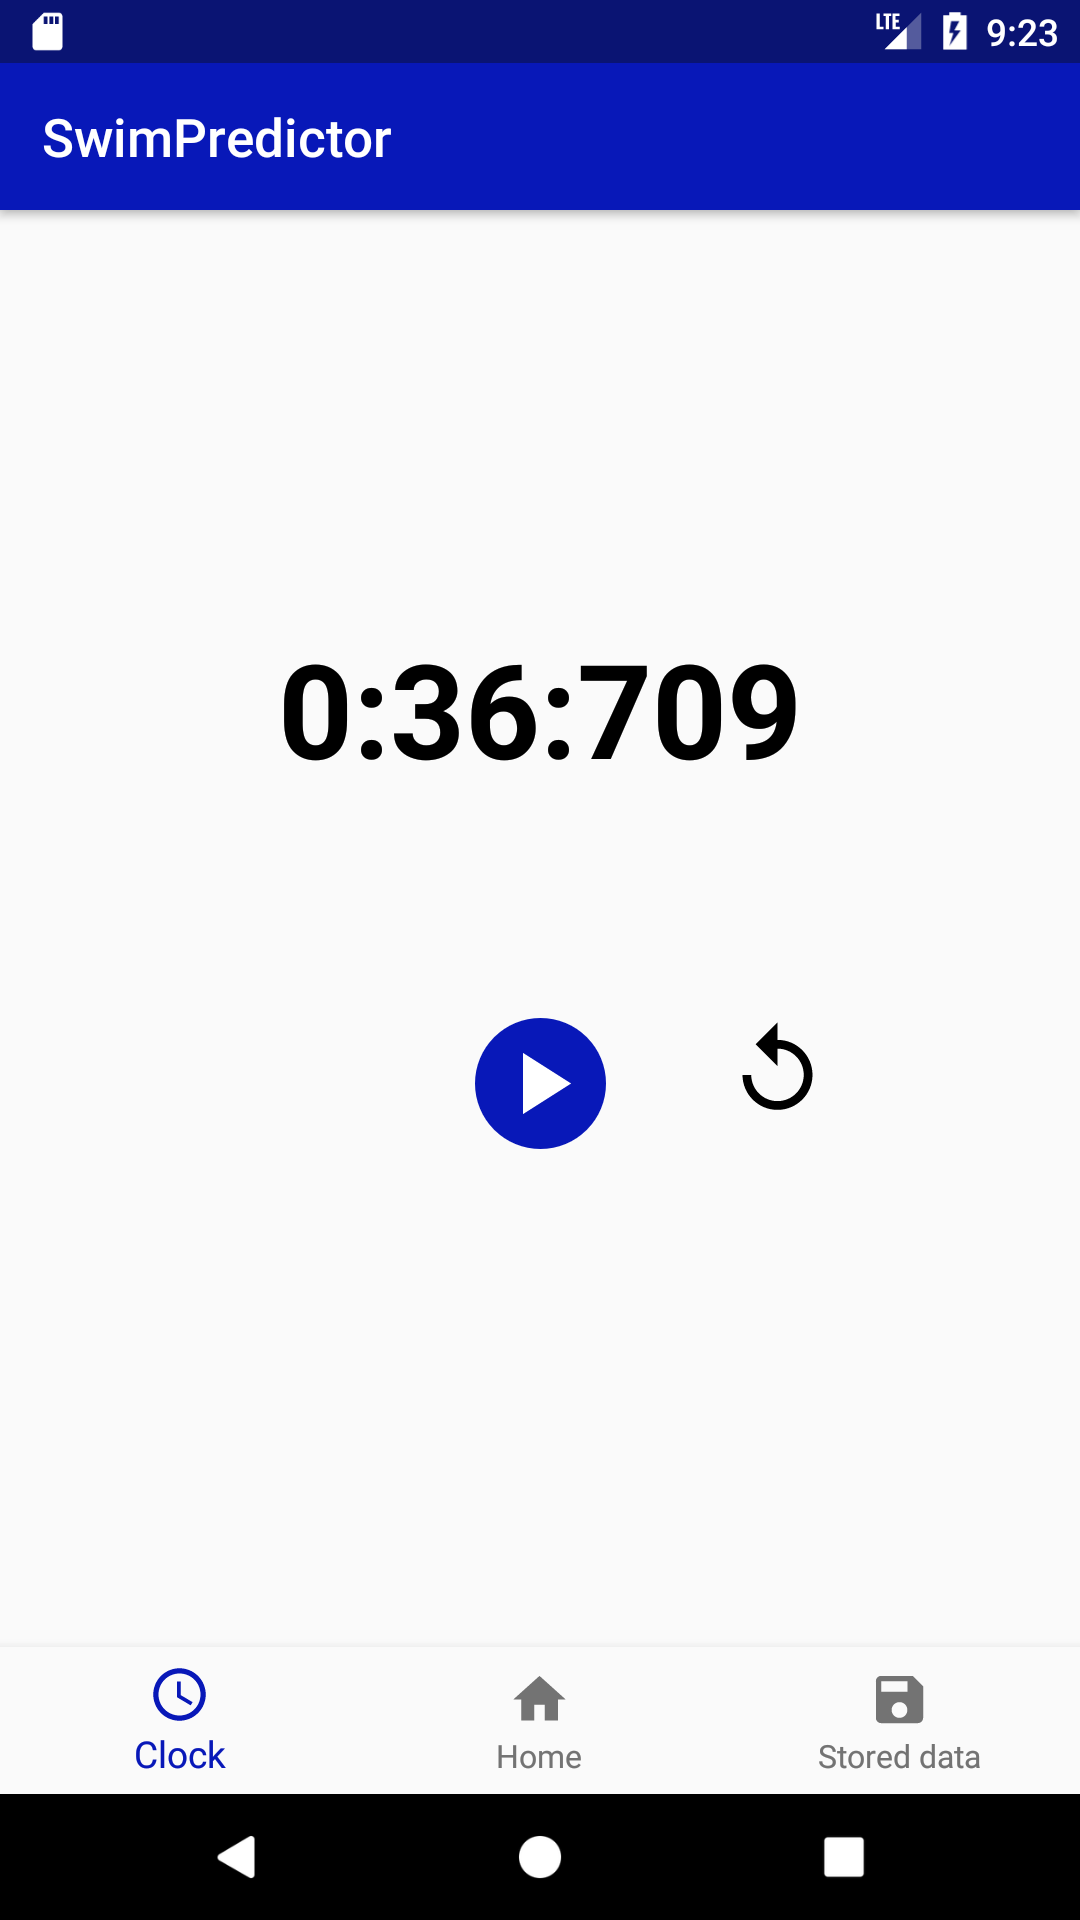
\includegraphics[width=\textwidth]{visualisation/stopwatch_view.png}
\end{minipage}
\begin{minipage}{0.2\textwidth}
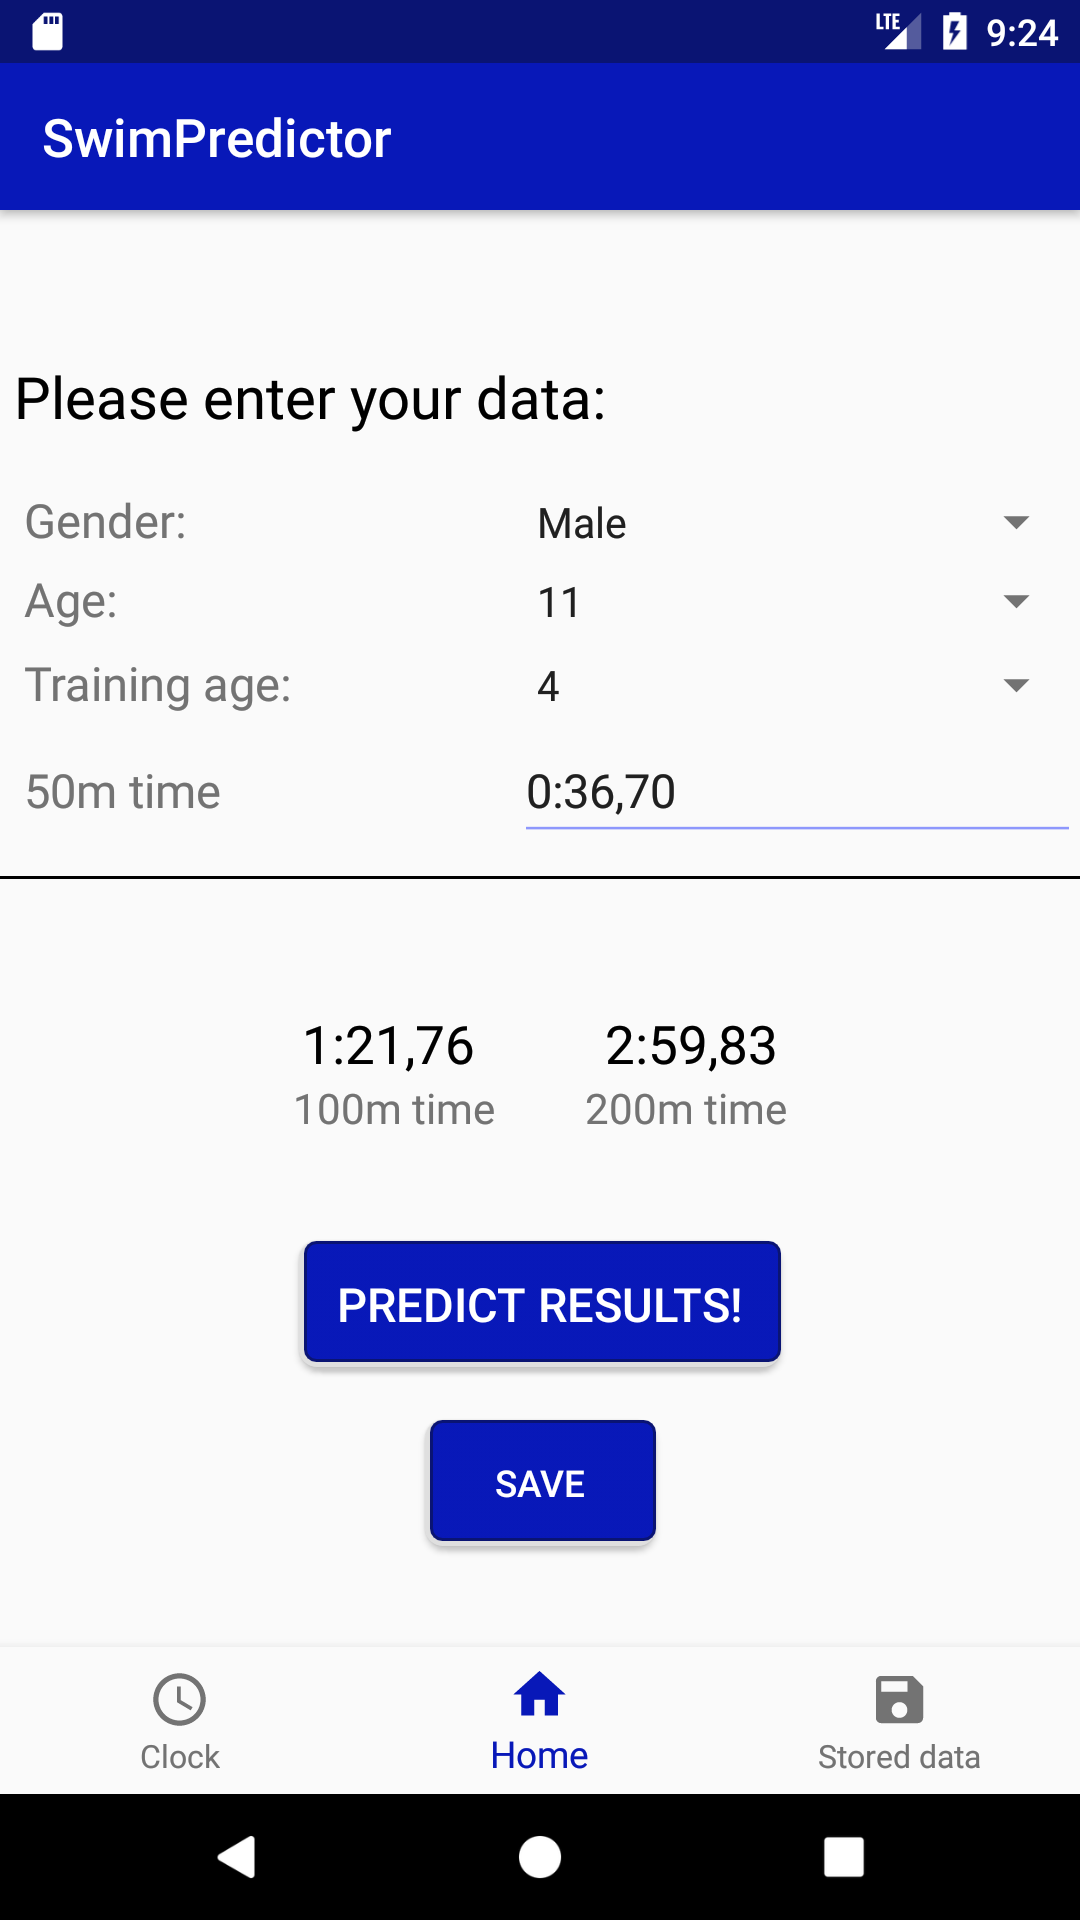
\includegraphics[width=\textwidth]{visualisation/prediction_view.png}
\end{minipage}
\caption{Screenshots of the app's stopwatch and home view}
\label{fig:app_screenshots}
\end{figure}
In the core or home fragment the coach can enter the information of the swimmer and the 50m time he measured in training and let the app predict the longer distance times based on this information. It loads the pre-trained tensorflow-lite model it needs for the predictions from the app's assets folder. To use these models, we need to include the tensorflow-lite library in our app's \texttt{build.gradle} file. The coach can enter the information about the swimmer by choosing values from a dropdown list. This prevents the coach from entering unknown values or values in the wrong format. Moreover, the core fragment has a predict button, with which the user can trigger the prediction, two text views to display the predicted times and a store button to store the current record.\\
The stopwatch function implemented in the \texttt{org.swimpredictor.ui.clock} package has two buttons, a play/pause button and a reset button, as well as a text to display the measured time. We explain the stopwatch logic in Figure \ref{fig:stopwatch_logic}. At first the stopwatch is set to zero. When the play button is clicked, the time starts to run and the play icon on the play/pause button changes to a pause icon. When clicking the pause button, the stopwatch stops running, displays the current time and the button shows the play icon again. The time is saved into a shared preference object and loaded into the 50m time field of the prediction view thus the user does not need to transfer the time himself. The stopwatch can be reset at any time. If the reset button is clicked, the displayed time and the time stored in the shared preferences are set to zero again. We simulate the running stopwatch using a java $Runnable$ object that displays the difference between the start time and the current system time \footnote{\url{https://www.android-examples.com/android-create-stopwatch-example-\ tutorial-in-android-studio/}, accessed 31.12.2019}.\\
\begin{figure}[ht]
    \centering
    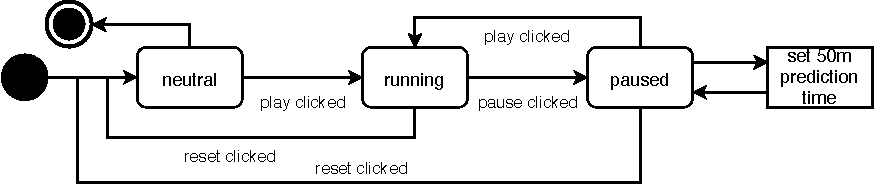
\includegraphics[scale=0.5]{visualisation/StopwatchLogic.pdf}
    \caption{Activity diagram for stopwatch function}
    \label{fig:stopwatch_logic}
\end{figure}
We implement the store functionality in the \texttt{org.swimprodictor.database} package using Android's Room \footnote{\url{https://developer.android.com/training/data-storage/room}, accessed 12.01.2020} and a SQLite database behind it. Although we only have one table, we consider a database the best way to store our data as it is rather easy to implement with Room and it assures consistency by built-in constraints. A \texttt{DataSample} object represents an entity in this table and contains all the information from the data records, as explained in section \ref{sec:data_gen}, together with a unique description that the coach enters when saving a record and human-readable String representation of the times. These Strings have the format \texttt{m:ss,dscs}, e.g. \texttt{1:23,45}. The database itself offers the functionality to insert and delete a sample. The database tab displays all samples stored in the database. We had problems to display the entries in the database as the number of entries in the database changes thus a static TableView is not applicable. Therefore, we use the Open-Source version of the SortableTableView\footnote{\url{https://github.com/ISchwarz23/SortableTableView}, accessed 12.01.2020}. Due to the small display on a mobile device, we were not able to show all information of all samples at the same time. Therefore, the table only shows the description and the three times. The remaining information about the swimmer can be shown in a pop- up message when clicking at the respective sample. To delete a sample, the user needs to long click on the sample he wants to delete. The app then requires a confirmation of the user. If he confirms the deletion, the sample is removed from the database, and the table is reloaded. Figure \ref{fig:app_screenshots_database} shows the TableView of the database entries as well as the pop-up messages with detailed information and deletion confirmation.
\begin{figure}[ht]
\begin{minipage}{0.15\textwidth}
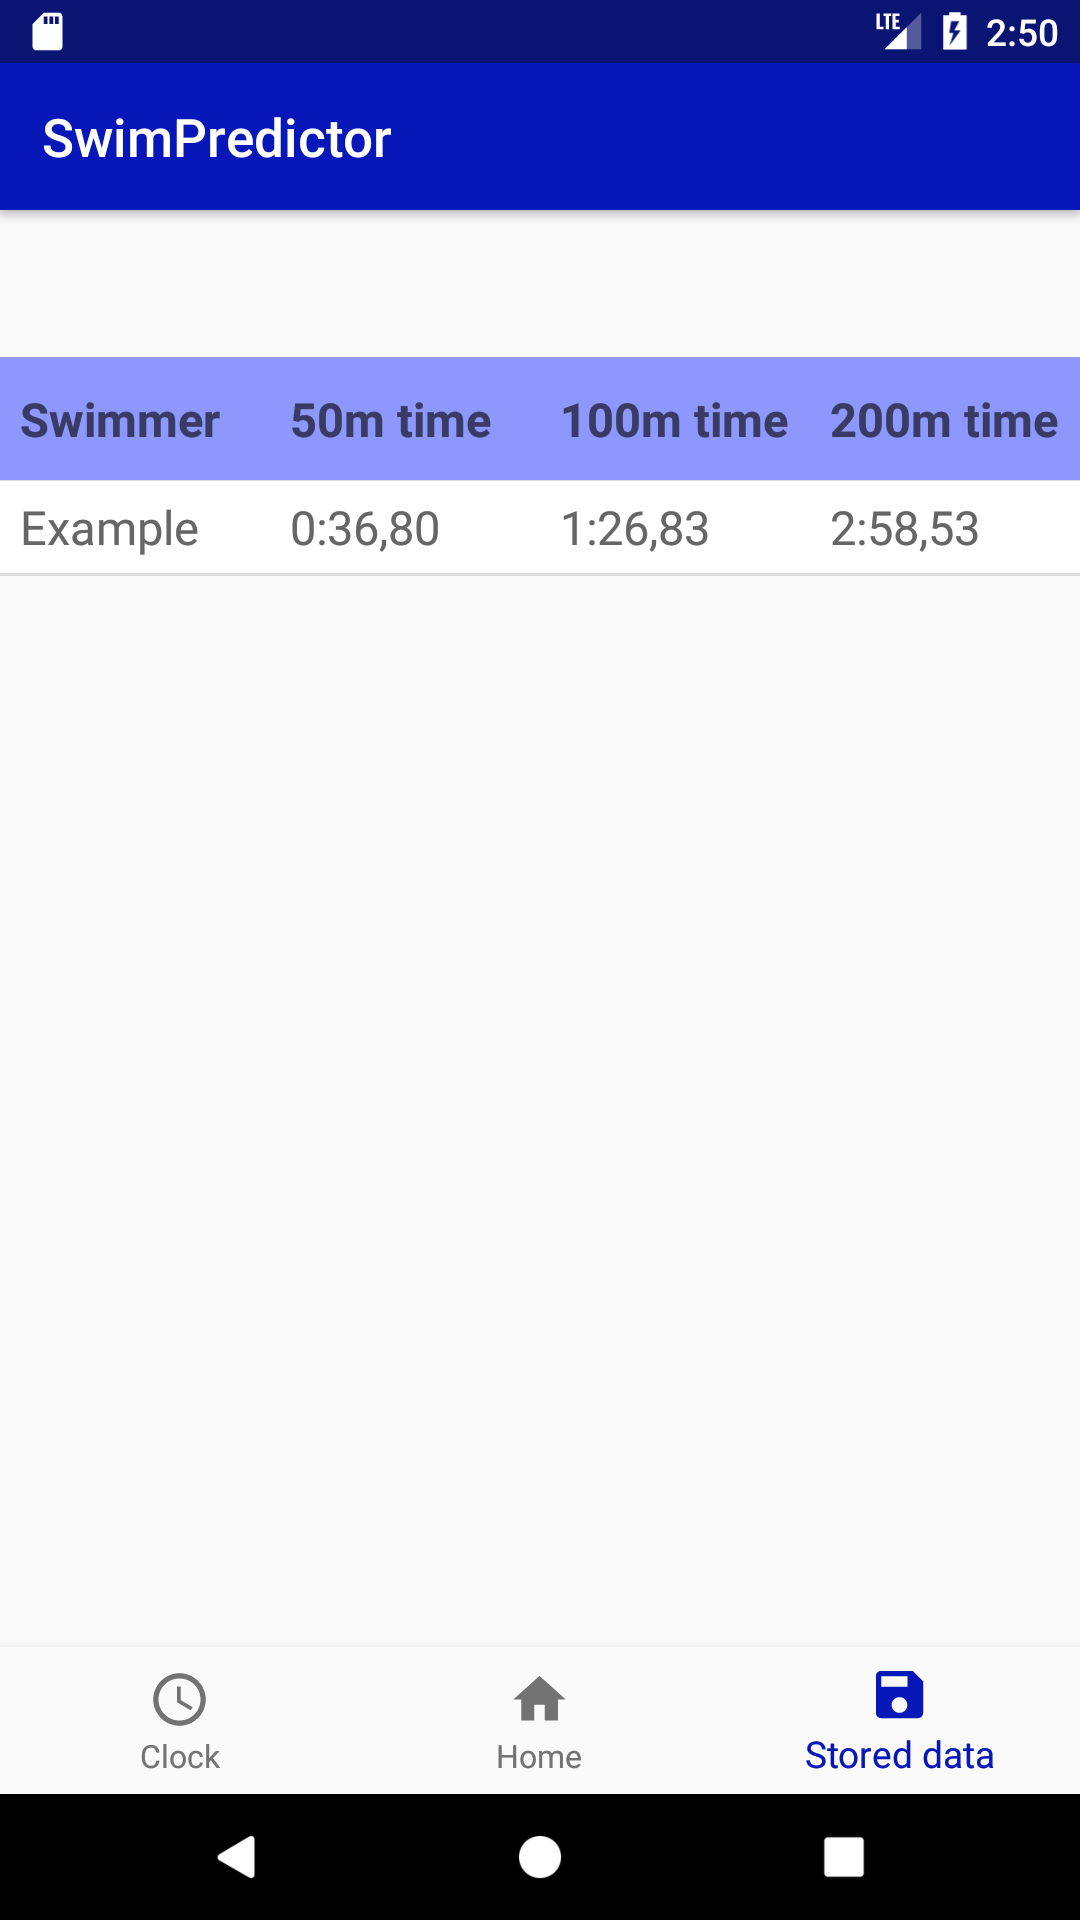
\includegraphics[width=\textwidth]{visualisation/database_view.png}
\end{minipage}
\begin{minipage}{0.15\textwidth}
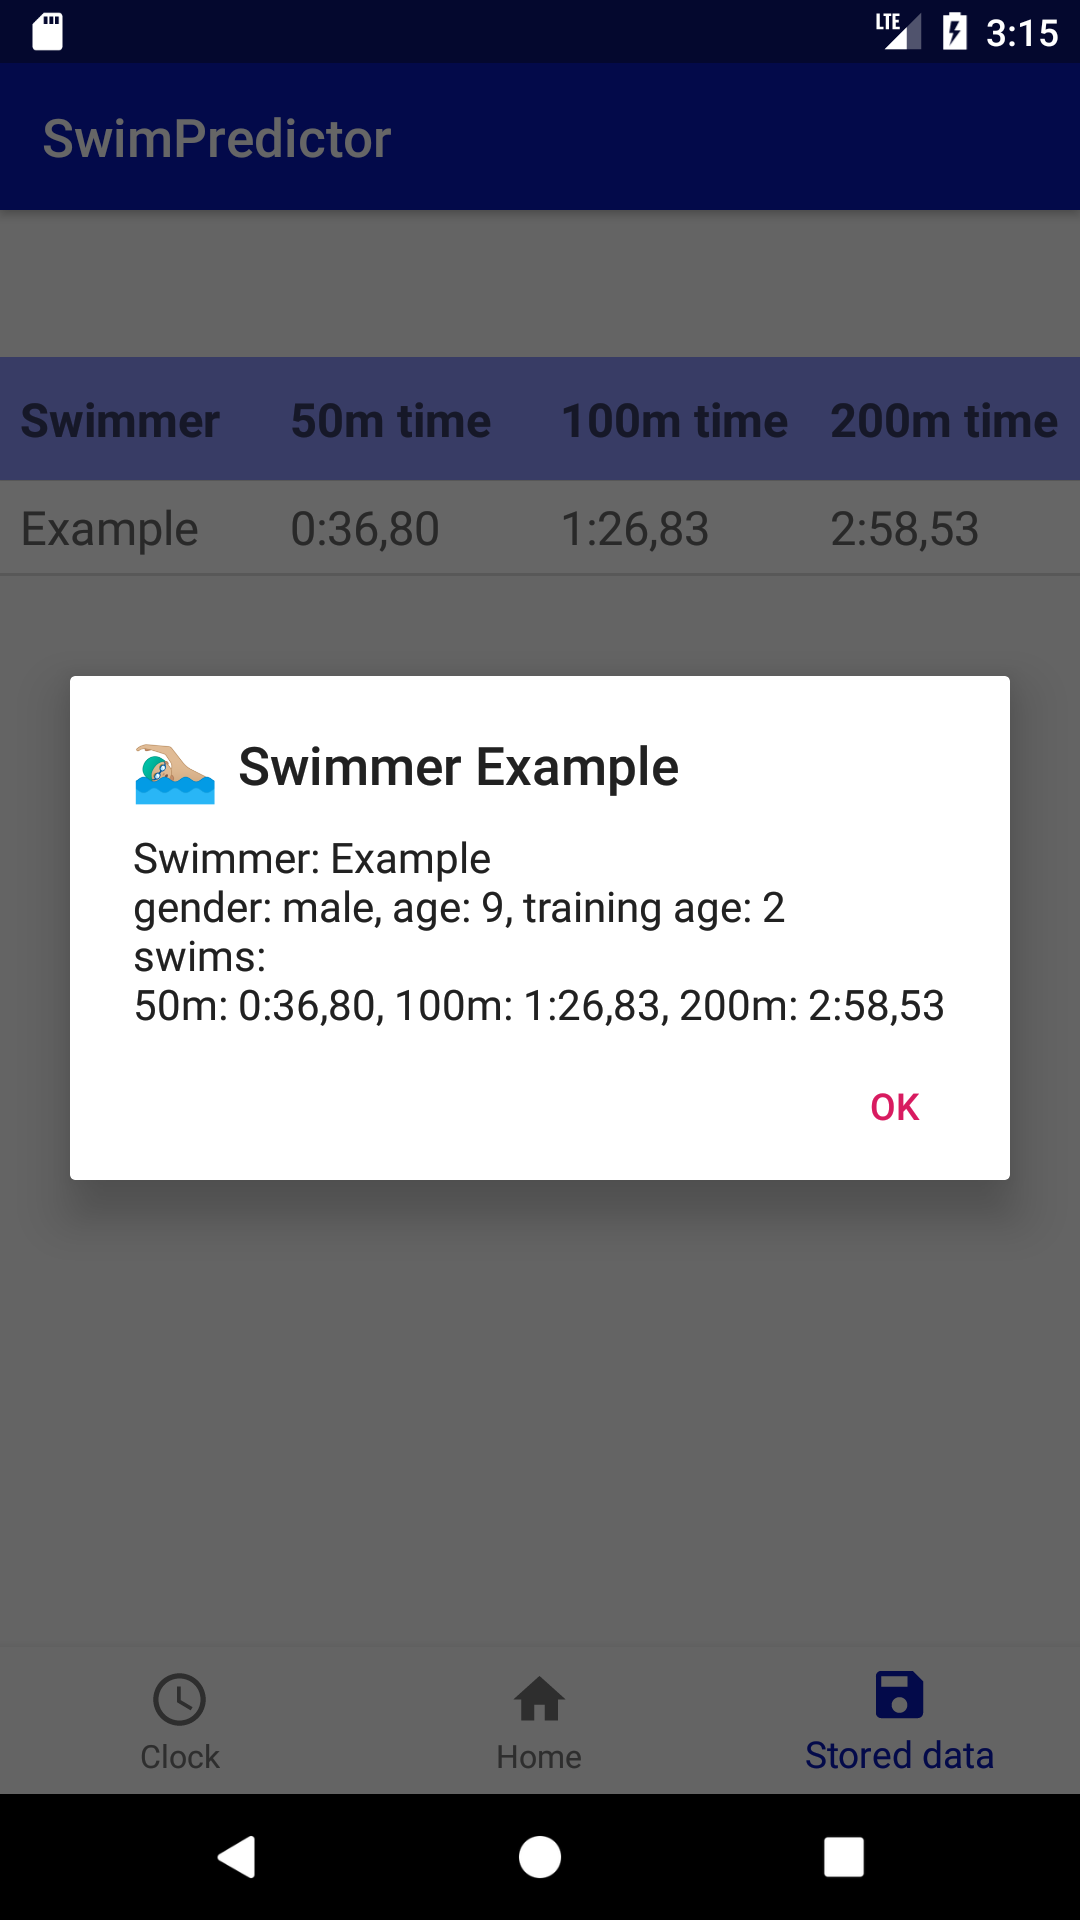
\includegraphics[width=\textwidth]{visualisation/app_detailed_information.png}
\end{minipage}
\begin{minipage}{0.15\textwidth}
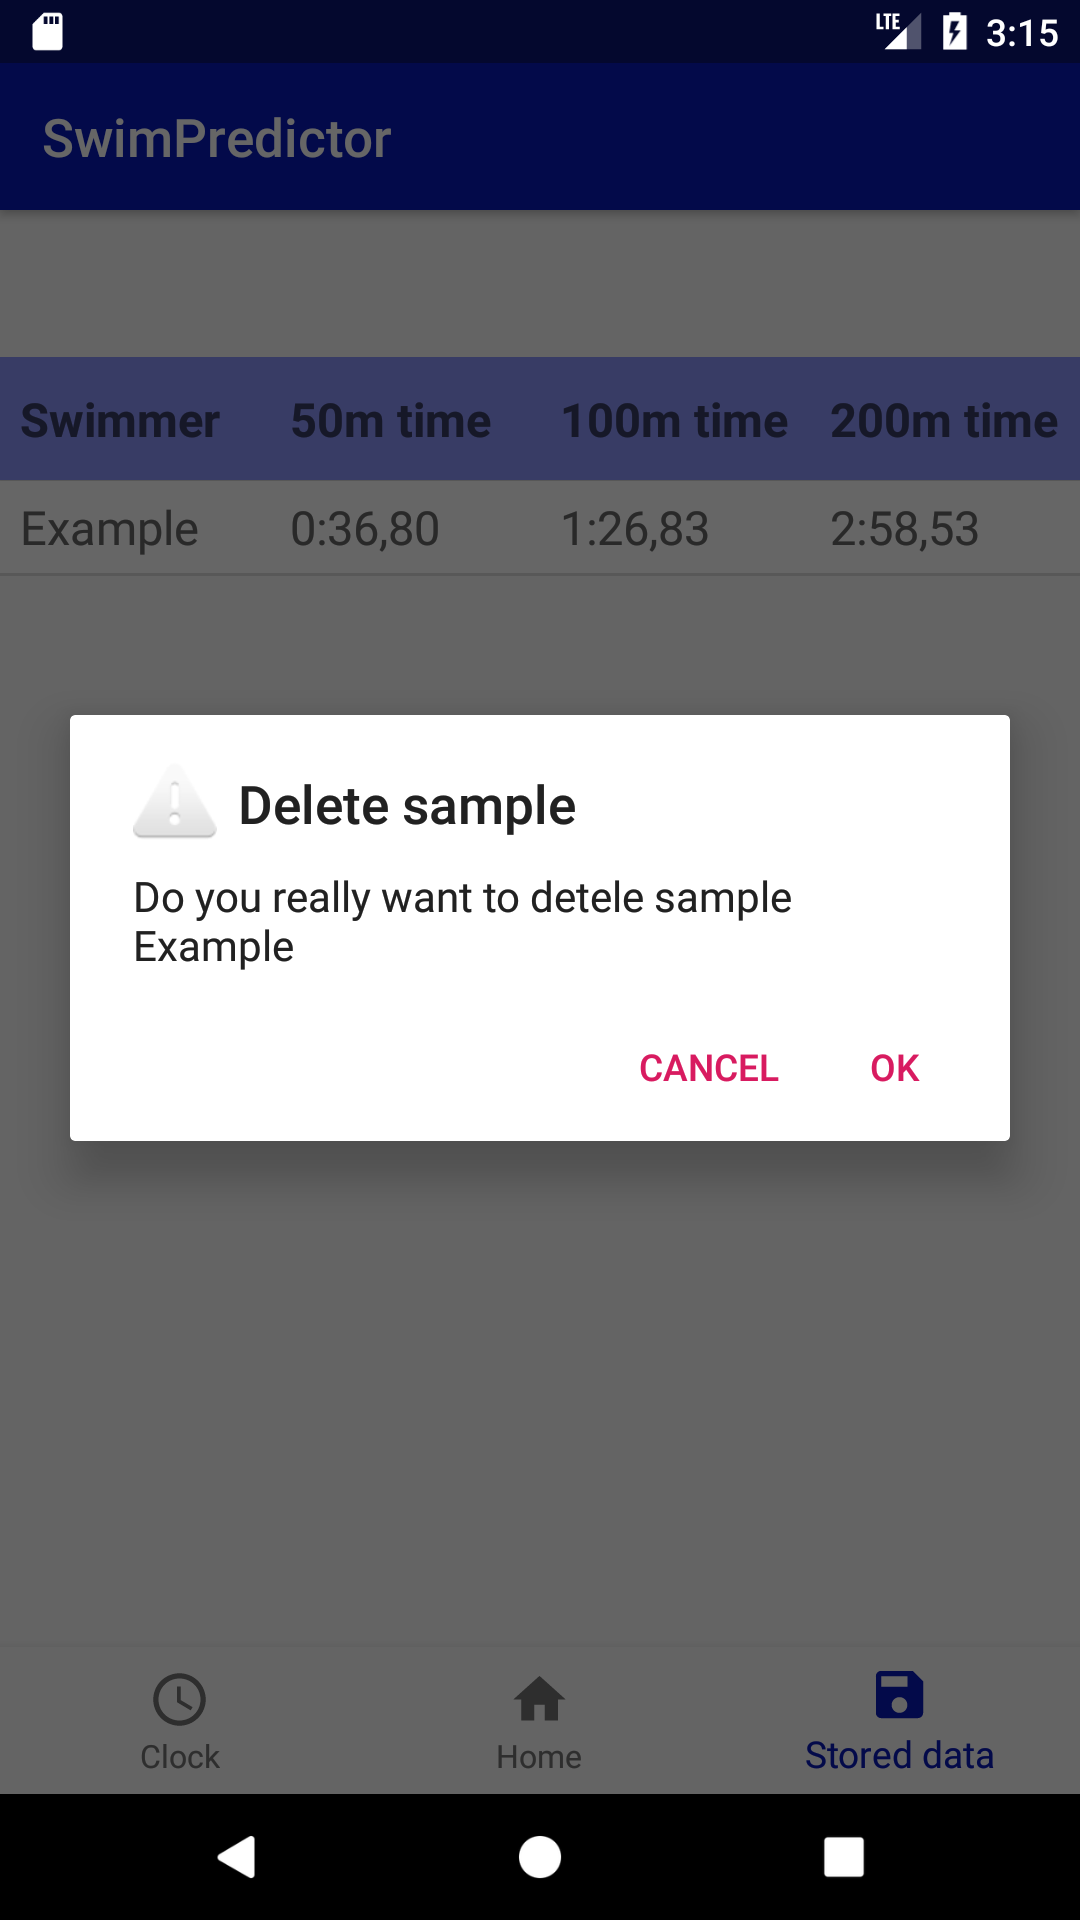
\includegraphics[width=\textwidth]{visualisation/app_confirm_deletion.png}
\end{minipage}
\caption{Screenshots of the app's database functionality}
\label{fig:app_screenshots_database}
\end{figure}